\documentclass{article}
\usepackage{amsmath, amssymb, amsbsy, tcolorbox, array, sfmath, enumerate, pgfplots, multicol}
\renewcommand{\familydefault}{\sfdefault}
\pgfplotsset{compat=newest}
\usetikzlibrary{arrows.meta}
\everymath{\displaystyle}
\tikzset{>=stealth}
\usepackage[top = 0.25in, bottom = 0.25in, left = 1in, right = 1in]{geometry}
\pagestyle{empty}
\raggedright

\newcounter{example}[section]
\newenvironment{example}[1][]{\refstepcounter{example}\par\medskip
   {\color{red}\textbf{Example~\theexample. #1}}}{\medskip}

\begin{document}

\section*{Operations With Functions}

\begin{tcolorbox}[colframe=orange!70!white, coltitle=black, title=\textbf{Summary}]
\begin{enumerate}
    \item Arithmetic operations with functions is very similar to arithmetic operations with numbers.
\end{enumerate}
\end{tcolorbox}
\bigskip 

We can add, subtract, multiply, and divide functions just like we can with real numbers.	\newline\\
\begin{center}
\setlength{\extrarowheight}{10pt}
\begin{tabular}{c|c}
 \textbf{Sum}    &  $(f+g)(x) = f(x) + g(x)$    \\[6pt]
 \hline
 \textbf{Difference}   &    $(f-g)(x)=f(x)-g(x)$    \\[6pt] 
 \hline
 \textbf{Product}   &   $(fg)(x)=f(x) \cdot g(x)$   \\[6pt]
 \hline
 \textbf{Quotient}  &   $\left(\dfrac{f}{g}\right)\left(x\right) = \dfrac{f(x)}{g(x)}$, \quad $g(x) \neq 0$   \\
\end{tabular}
\end{center}
\bigskip 

So if $f(x) = x+2$ and $g(x) = x^2 - 4$, then 
\begin{align*}
    (f+g)(x) &= {\color{red}f(x)} + {\color{blue}g(x)} \\
    &=  {\color{red}x+2} + {\color{blue}x^2 - 4}   \\
    &=x^2 +x - 2  
\end{align*}
\smallskip 

\begin{example}
Find each of the following if $f(x) = x^2 + 2x - 3$ and $g(x) = x-1$ 
\begin{enumerate}[(a)]
\begin{multicols}{3}
    \item $(f + g)(x)$
    \item $(f - g)(x)$
    \item $(g - f)(x)$
\end{multicols}
\vfill 
\begin{multicols}{3}
    \item $(fg)(x)$
    \item $\left(\dfrac{f}{g}\right)(x)$
    \item $\left(\dfrac{g}{f}\right)(x)$
\end{multicols}
\vfill 
\end{enumerate}
\end{example}

\newpage 

\subsection*{Evaluating the Sum, Difference, Product, or Quotient of Two Functions}

If $f(x) = x+2$ and $g(x) = x^2-4$, then
\begin{align*}
(f+g)(3) &= f(3) + g(3) \\
&= (3+2) + (3^2-4) \\
&= 10
\end{align*}
\smallskip 

\begin{example}
Evaluate each of the following if $f(x) = x^2 - 3$ and $g(x) = 4x + 5$
\begin{multicols}{3}
\begin{enumerate}[(a)]
    \item $(f + g)(3)$   
    \item $(f - g)(0)$   
    \item $(fg)(2)$      
\end{enumerate}
\end{multicols}
\vfill 
\begin{multicols}{3}
\begin{enumerate}[(a)] \setcounter{enumi}{3}
    \item $(gg)(1)$      
    \item $\left(\dfrac{f}{g}\right)(1)$     
    \item $\left(\dfrac{g}{f}\right)(8)$     
\end{enumerate}
\end{multicols}
\end{example}
\vfill 


\subsection*{Tabular and Visual Methods}

\begin{example} 
Find each given the table below.
\begin{center}
\begin{tabular}{c|c|c|c|c|c|c|c}
    $\pmb{x}$ & $\pmb{-3}$ & $\pmb{-2}$ & $\pmb{-1}$ & \textbf{0} & \textbf{1} & \textbf{2} & \textbf{3} \\ \hline 
    $\pmb{f(x)}$ & 1 & $-2$ & $-3$ & $-1$ & 3 & 2 & 0 \\ \hline
    $\pmb{g(x)}$ & $-2$ & 2 & $-3$ & 3 & 0 & 1 & $-1$ \\
\end{tabular}
\end{center}
\begin{multicols}{4}
\begin{enumerate}[(a)]
    \item $(f + g)(-1)$
    \item $(f - g)(2)$
    \item $(fg)(0)$
    \item $\left(\frac{g}{f}\right)(-3)$
\end{enumerate}
\end{multicols}
\end{example}
\vfill 
\begin{example}
Find each given the graph below.
\begin{center}
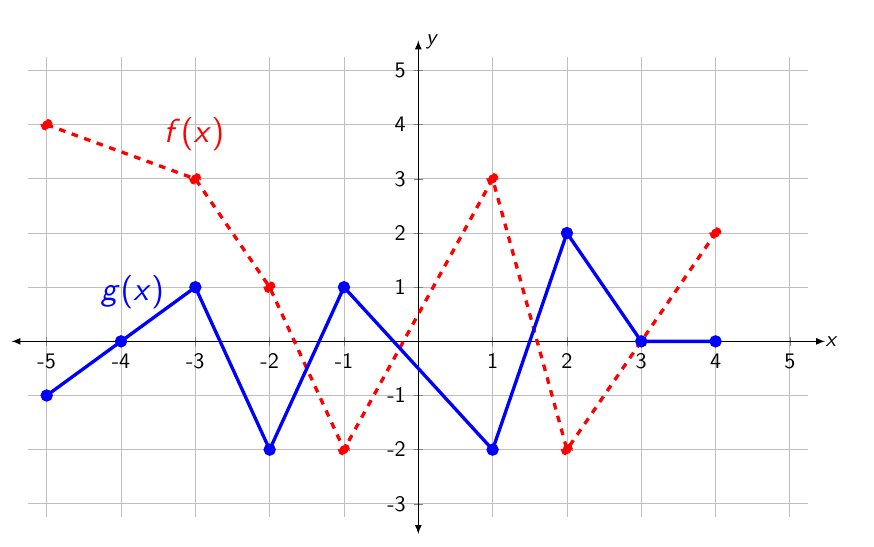
\begin{tikzpicture}[scale=0.8]
\begin{axis}
[   
    grid,
    axis lines=middle,
    xmin=-5.25,xmax=5.25,
    ymin=-3.25,ymax=5.25,
    restrict y to domain=-3:5,
    xtick={-5,-4,...,5},
    xticklabels={-5,-4,-3,-2,-1,,1,2,3,4,5},
    ytick={-3,-2,...,5},
    yticklabels={-3,-2,-1,,1,2,3,4,5},
    axis line style={latex-latex},
    axis line style={shorten >=-7.5pt, shorten <=-7.5pt},
    xlabel=$x$,
    ylabel=$y$,
    xlabel style={at={(ticklabel* cs:1)},anchor=west, xshift=0.15cm},
    ylabel style={at={(ticklabel* cs:1)},anchor=south west},
    width=5.5in,
    height=3.5in
]
\addplot[mark = *, color=red, line width = 1.5, dashed] coordinates
{
    (-5,4)
    (-3,3)
    (-2,1)
    (-1,-2)
    (1,3)
    (2,-2)
    (4,2)
};
\addplot[mark=*, color=blue, line width = 1.5] coordinates
{
    (-5,-1)
    (-4,0)  
    (-3,1)
    (-2,-2)
    (-1,1)
    (1,-2)
    (2,2)
    (3,0)
    (4,0)
};
\end{axis}
\node at (2.0,6.5) [anchor = north west] {\color{red} \large $f(x)$};
\node at (1,4) [anchor = north west] {\color{blue} \large $g(x)$};
\end{tikzpicture}
\end{center}
\begin{multicols}{4}
\begin{enumerate}[(a)]
    \item $(f+g)(-5)$
    \item $(g-f)(-2)$
    \item $(fg)(4)$
    \item $\textstyle \left(\frac{f}{g}\right)(1)$
\end{enumerate}
\end{multicols}
\end{example}
\vfill 
\end{document}
